\chapter{Introduction}
\label{ch1_introduction}
\section{Motivation}
\label{sect1_1}
Moore’s legendary law: "The number of transistors and resistors on a chip doubles every 18 months," which predicts the pace of technology scaling is largely mistranslated to imply CPU performance. Although conventional scaling techniques have challenged the tacit promises of performance put forth by Moore, Intel - co-founded by Moore himself - has found novel ways to steadily stride along his prognosis, an achievement that can be attributed to a legion of engineers. However, as we approached infinitesimally small-sized transistors, we chalked up paltry performance gains and came to terms with the fact that purely upgrading hardware generations is not the solution. 
\newline \newline
The Figure \ref{fig:sematech} illustrates the gap between the computational demand with increasing complexity and the actual productivity. Increasing the operating frequency or the number of cores does not yield the performance desired from the current complex, compute-intensive applications. \newline \newline
\begin{figure}[h!]
  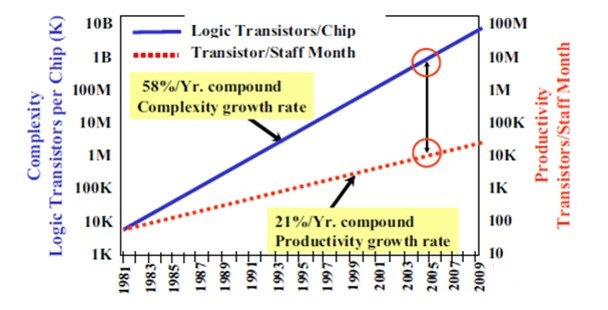
\includegraphics[width=\linewidth]{figures/sematech.jpg}
  \caption{The Productivity Gap
  \cite{industry1999international}}
  \label{fig:sematech}
\end{figure}
This calls for multi-core systems that achieve the desired performance by integrating specialized processing abilities required for specific tasks. Heterogeneous system architectures exploit multiple processor types, to realize the best of both data-parallel and task-parallel (sequential) applications \cite{amd_resources}.\newline \newline
To realize the full potential of such systems, the system designers should scrupulously integrate the diverse compute elements available in the platform and allow them to work together seamlessly. While conventional accelerators limit productivity by demanding high skills in hardware engineering, heterogeneous architectures having GPPs and specialized co-processors offer software-like programmability, enhanced application portability and consequently, improved productivity. Some of the popular heterogeneous computing platforms include network processors such as Intel IXP, Embedded systems such as TI OMAP, NVIDIA Tegra and Apple A9, Reconfigurable devices such as Xilinx FPGAs (Virtex, Kintex, etc.) in Zynq platform containing dual core ARM Cortex A9 Processors, General purpose processors such as IBM Cell and ARM big.LITTLE CPU architectures \cite{wiki_nanoscale}. \newline \newline
These devices guarantee a power-aware design with increased data parallelism and throughput. However, we should also be mindful of the challenges they pose such as different instruction set architectures for different compute elements, varying cache structure and coherence protocols, varying memory access patterns (uniform or non-uniform) and interface types, etc. \cite{wiki_nanoscale} Opaque programming paradigms (like POSIX standard for threads), the differences in underlying micro-architecture and abstractions associated with high-level language programming can impede performance predictions and sometimes, increase power consumption. Designers should explicitly handle thread synchronizations and shared variable protection in multi-threaded applications and partition the application suitably between various computing elements. Example: Running a sequential task on FPGA leads to under-utilization of resources and slows down the performance. Similarly, performing SIMD operations such as vector/ array processing on a CPU would be a bad choice. Design decisions generally involve domain expertise and design space exploration, which is a quantitative approach to recognizing the design variables with the most beneficial effect on the system’s performance goals. \newline \newline
To mitigate the challenges listed above, we need to establish a standard programming model that is portable across devices and capable of delivering the desired performance. 
For simple applications, design decisions are straightforward. This prompts us to explore some complex, compute-intensive applications and study the impact of various design decisions on their performance. This report intends to investigate two such applications, namely MNIST Digit classifier using Convolutional Neural Network, and Fully Homomorphic Encryption scheme, and optimize them to achieve the best-case acceleration on a heterogeneous platform. 

\section{Contribution}
\label{sect1_2}
The primary focus areas of this thesis can be summarized as follows:
\begin{itemize}
\item Identification and understanding of two applications of high computational complexity which show potential for hardware acceleration.
\item Understanding of programming models best suited for the parallelization of the identified complex applications.
\item Profiling various parts of the applications to isolate the critical paths that need improvements.
\item Performing architectural exploration and suitably partitioning the application between various compute elements available in the platform.
\item Running and profiling the applications to study the performance improvements with the modified design.
\end{itemize}
\section{Organization}
\label{sect1_3}
The report consists of the following chapters: 
\textbf{Chapter \ref{ch2_background}} presents background software knowledge and hardware requirements needed for this project.
\textbf{Chapter \ref{ch3_lit_review}} studies an implementation of OpenCL platform and its features. Few details of the LeNet-5 architecture of Convolutional Neural Networks are also explained. The chapter continues to discuss previously used ISAs and the need for a new ISA which was met by RISC-V. Implementations of processors based on this architecture are also seen here.
\textbf{Chapter \ref{ch4_opencl}} explains in detail how OpenCL capitalises on devices with parallel programming capabilities. A few simple experiments are conducted to demonstrate how optimum results can be achieved. 
\textbf{Chapter \ref{ch5_cnn}} throws light into the field of neural networks, exploring few models of neural networks. The work of Lecun, Y. in the field of character recognition using \ac{CNN} and Deep Learning is discussed in detail. An existing application is analysed and profiled on multiple devices.
\textbf{Chapter \ref{ch6_riscv}} shows how an open-source architecture would benefit the evolution of technology. RISC-V is studied as the architecture to be used for the development of a hypothetical accelerator consisting of a network of individual processors. The implementation of a new processor based on this ISA is discussed and explained in detail. 
We thereby conclude in \textbf{Chapter \ref{ch7_conclusion}} and discuss work to be done in the future.